% =====================================================================
%  PRESENTACION-CVRP.TEX
%  Presentación final del trabajo de investigación:
%  CVRP — Método Exacto (Informe 1) vs. Particle Swarm Optimization (Informe 2).
%
%  Optimización en Ingeniería — Magíster en Ingeniería Informática USACH 2026.
%  Profesores: Dra. Mónica Villanueva I. y Dr. Mario Inostroza P.
%  Autor: Cristopher Angulo Ahumada.
%
%  Pauta (enunciado, punto 9): presentación de no más de 20 minutos con los
%  principales resultados de AMBAS partes del curso y su comparativa.
%
%  Plantilla (preámbulo/estilo) reutilizada de las presentaciones previas
%  (GRU / PSO paper). Para cambiar el esquema de color, editar SOLO los
%  tres colores de "Paleta".
%  Compilación:  pdflatex main.tex   (x2)
% =====================================================================

\documentclass[aspectratio=169, 11pt, xcolor={dvipsnames,table}]{beamer}

% ── Paquetes base ────────────────────────────────────────────────────
\usepackage[utf8]{inputenc}
\usepackage[T1]{fontenc}
\usepackage[spanish, es-tabla]{babel}
\usepackage{lmodern}
\usepackage{microtype}
\usepackage{amsmath, amssymb, mathtools, bm}
\usepackage{graphicx}
\usepackage{booktabs, array, multirow}
\usepackage{multicol}
\usepackage{caption}
\captionsetup{font=footnotesize, labelfont=bf}
\usepackage{tcolorbox}
\tcbuselibrary{skins}
\usepackage{algorithm}
\usepackage{algpseudocode}
\floatname{algorithm}{Algoritmo}
\renewcommand{\algorithmicrequire}{\textbf{Entrada:}}
\renewcommand{\algorithmicensure}{\textbf{Salida:}}
\usepackage{tikz}
\usetikzlibrary{positioning, arrows.meta, calc, shapes.geometric, shapes.misc, fit, backgrounds}
\hypersetup{hidelinks}
\usepackage{xcolor}

% ── Paleta (identidad propia; edita SOLO estos tres colores) ─────────
\definecolor{TemaPrimario}{RGB}{14,92,74}    % verde petróleo (0E5C4A) -> barras de título
\definecolor{TemaAcento}{RGB}{199,124,30}    % ámbar/ocre (C77C1E)     -> bloques de alerta
\definecolor{TemaNeutro}{RGB}{55,71,79}      % pizarra (37474F)        -> bloques de ejemplo
\colorlet{UsachAzul}{TemaPrimario}
\colorlet{UsachNaranja}{TemaAcento}
\colorlet{UsachGris}{TemaNeutro}
\definecolor{UsachGrisClaro}{RGB}{230,230,230}

% ── Theme + colores Beamer ───────────────────────────────────────────
\usetheme{Madrid}
\useinnertheme{rectangles}
\useoutertheme{infolines}
\setbeamertemplate{headline}{}
\setbeamertemplate{navigation symbols}{}
\setlength{\medskipamount}{3pt plus 1pt minus 1pt}
\setbeamersize{text margin left=5mm, text margin right=5mm}

\makeatletter
\let\beamer@@frameORIG\beamer@@frame
\def\beamer@@frame[#1]{\beamer@@frameORIG[shrink=55,#1]}
\makeatother

\setbeamertemplate{footline}{%
  \leavevmode%
  \hbox{%
  \begin{beamercolorbox}[wd=.33\paperwidth,ht=2.25ex,dp=1ex,center]{author in head/foot}%
    \usebeamerfont{author in head/foot}\insertshortauthor
  \end{beamercolorbox}%
  \begin{beamercolorbox}[wd=.34\paperwidth,ht=2.25ex,dp=1ex,center]{title in head/foot}%
    \usebeamerfont{title in head/foot}\insertshorttitle
  \end{beamercolorbox}%
  \begin{beamercolorbox}[wd=.33\paperwidth,ht=2.25ex,dp=1ex,right]{date in head/foot}%
    \usebeamerfont{date in head/foot}\insertshortdate{}\hspace*{2em}
    \insertframenumber{} / \inserttotalframenumber\hspace*{2ex}
  \end{beamercolorbox}}%
  \vskip0pt%
}

\setbeamercolor{structure}{fg=UsachAzul}
\setbeamercolor{palette primary}{bg=UsachAzul, fg=white}
\setbeamercolor{palette secondary}{bg=UsachAzul!80, fg=white}
\setbeamercolor{palette tertiary}{bg=UsachAzul, fg=white}
\setbeamercolor{title}{fg=UsachAzul, bg=white}
\setbeamercolor{frametitle}{fg=white, bg=UsachAzul}
\setbeamercolor{section in head/foot}{bg=UsachAzul, fg=white}
\setbeamercolor{subsection in head/foot}{bg=UsachAzul!80, fg=white}
\setbeamercolor{author in head/foot}{bg=UsachAzul, fg=white}
\setbeamercolor{title in head/foot}{bg=UsachAzul!85, fg=white}
\setbeamercolor{date in head/foot}{bg=UsachAzul, fg=white}
\setbeamercolor{itemize item}{fg=UsachNaranja}
\setbeamercolor{itemize subitem}{fg=UsachNaranja!80}
\setbeamercolor{enumerate item}{fg=UsachNaranja}
\setbeamercolor{block title}{bg=UsachAzul, fg=white}
\setbeamercolor{block body}{bg=UsachAzul!5, fg=black}
\setbeamercolor{block title alerted}{bg=UsachNaranja, fg=white}
\setbeamercolor{block body alerted}{bg=UsachNaranja!8, fg=black}
\setbeamercolor{block title example}{bg=UsachGris, fg=white}
\setbeamercolor{block body example}{bg=UsachGris!8, fg=black}
\setbeamercovered{transparent=25}
\usefonttheme[onlymath]{serif}

\newcommand{\azul}[1]{\textcolor{UsachAzul}{#1}}
\newcommand{\naranja}[1]{\textcolor{UsachNaranja}{#1}}
\newcommand{\gris}[1]{\textcolor{UsachGris}{#1}}

% ── Atajos de notación ───────────────────────────────────────────────
\newcommand{\xx}{\mathbf{x}_i}
\newcommand{\vv}{\mathbf{v}_i}
\newcommand{\pp}{\mathbf{p}_i}
\newcommand{\pg}{\mathbf{p}_g}

% ── Cajas ────────────────────────────────────────────────────────────
\newtcolorbox{ideaclave}[1][]{
  colback=UsachNaranja!8, colframe=UsachNaranja!80!black,
  fonttitle=\bfseries, title=Idea clave, #1}
\newtcolorbox{paperbox}[1][]{
  colback=UsachGris!8, colframe=UsachGris,
  fonttitle=\bfseries, title=En el informe, #1}

% ── Metadatos ────────────────────────────────────────────────────────
\title[CVRP: Exacto vs.\ PSO]{\textbf{CVRP: Método Exacto vs.\ Particle Swarm Optimization}}
\subtitle{Trabajo de investigación --- Informes 1 y 2}
\author[Angulo]{Cristopher Angulo Ahumada}
\institute[USACH]{%
  \footnotesize Optimización en Ingeniería \;\textbullet\; Profs.\ Dra.\ Mónica Villanueva I.\ y Dr.\ Mario Inostroza P.}
\date{Julio de 2026}

% =====================================================================
\begin{document}
% =====================================================================

% ─── PORTADA ─────────────────────────────────────────────────────────
{
\setbeamertemplate{background}{%
  \begin{tikzpicture}[remember picture, overlay]
    \fill[UsachAzul] (current page.north west) rectangle ([yshift=-1.6cm]current page.north east);
    \fill[UsachNaranja] ([yshift=-1.6cm]current page.north west) rectangle ([yshift=-1.75cm]current page.north east);
    \fill[UsachGris] ([yshift=0.55cm]current page.south west) rectangle ([yshift=0.65cm]current page.south east);
    \node[anchor=north west, xshift=7mm, yshift=-3.5mm]
      at (current page.north west) {
\includegraphics[height=9mm]{figuras/logo_diinf_blanco.png}};
    \node[anchor=north east, xshift=-8mm, yshift=-6mm, font=\footnotesize, text=white, align=right]
      at (current page.north east)
      {Magíster en Ingeniería Informática \;\textbullet\; Optimización en Ingeniería 2026};
  \end{tikzpicture}}
\setbeamertemplate{footline}{}
\begin{frame}[plain,noframenumbering]
  \vspace*{1.2cm}
  \titlepage
  \begin{center}\footnotesize\gris{%
  Método exacto: Laporte \& Nobert (1983) + cortes RCI \;\textbullet\; Metaheurística: PSO con representación SR-1 (Ai \& Kachitvichyanukul, 2009)}
  \end{center}
\end{frame}
}

% ─── CONTENIDO ───────────────────────────────────────────────────────
\begin{frame}{Contenido}
    \begin{center}\tableofcontents\end{center}
\end{frame}

\AtBeginSection[]{%
  \begin{frame}[plain,noframenumbering]
    \vspace*{2.5cm}\centering
    {\color{UsachAzul}\Huge\bfseries\insertsectionhead\par}
    \vspace{0.6cm}
    \textcolor{UsachNaranja}{\rule{0.25\textwidth}{2.5pt}}
    \vfill
  \end{frame}}

% =====================================================================
\section{El problema: CVRP}
% =====================================================================

\begin{frame}{El CVRP en una imagen}
\begin{columns}[c]
\column{0.56\textwidth}
\centering
\begin{tikzpicture}[font=\scriptsize, scale=0.92, >=Stealth]
  % deposito y clientes (siempre visibles)
  \node[star, star points=5, star point ratio=0.5, fill=UsachNaranja,
        draw=UsachNaranja!80!black, minimum size=16pt, inner sep=0pt] (dep) at (3.1,2.4) {};
  \node[below=0pt of dep, font=\tiny] {depósito};
  \foreach \i/\x/\y in {1/0.6/4.0, 2/1.5/4.5, 3/0.4/3.0, 4/1.4/2.2,
                        5/4.8/4.3, 6/5.6/3.4, 7/5.0/2.6,
                        8/1.2/0.7, 9/2.6/0.4, 10/4.4/0.8}{
    \fill[UsachGris] (\x,\y) circle (2.4pt);
  }
  % demandas de una ruta (aparecen con la ruta 1)
  \only<2->{
    \draw[UsachAzul, line width=1.2pt] (dep.center) -- (1.5,4.5) -- (0.6,4.0) -- (0.4,3.0) -- (1.4,2.2) -- (dep.center);
    \node[text=UsachAzul, font=\tiny] at (0.6,4.35) {$d=7$};
    \node[text=UsachAzul, font=\tiny] at (1.9,4.6) {$d=5$};
  }
  \only<3->{
    \draw[UsachNaranja!85!black, line width=1.2pt] (dep.center) -- (4.8,4.3) -- (5.6,3.4) -- (5.0,2.6) -- (dep.center);
  }
  \only<4->{
    \draw[UsachGris!80!black, line width=1.2pt] (dep.center) -- (1.2,0.7) -- (2.6,0.4) -- (4.4,0.8) -- (dep.center);
  }
\end{tikzpicture}
\column{0.44\textwidth}
\footnotesize
\begin{block}{Los datos}
$n$ clientes con \azul{demanda conocida}, un depósito, y $m$ vehículos idénticos de \azul{capacidad limitada} $D$.
\end{block}
\only<2->{\begin{exampleblock}{La decisión}
Diseñar \textbf{rutas} que partan y vuelvan al depósito, visiten a \textbf{cada cliente exactamente una vez}\ldots
\end{exampleblock}}
\only<3->{\begin{alertblock}{Las restricciones}
\ldots sin que la demanda acumulada de una ruta exceda $D$, \naranja{minimizando la distancia total}.
\end{alertblock}}
\end{columns}
\vspace{2pt}
\only<4->{\begin{ideaclave}
\scriptsize
El CVRP es \textbf{NP-hard}: combina \azul{particionar} clientes en rutas y \azul{ordenar} las visitas dentro de cada una. Por eso el curso lo aborda dos veces: método \textbf{exacto} (Informe 1) y \textbf{metaheurística} (Informe 2).
\end{ideaclave}}
\end{frame}

\begin{frame}{Formulación y datos experimentales}
\begin{columns}[c]
\column{0.5\textwidth}
\begin{block}{Función objetivo}
\footnotesize
Minimizar la distancia total recorrida por la flota:
\[ \min \; z = \sum_{r \in \mathcal{R}} \sum_{\{i,j\} \in r} c_{ij} \]
sujeto a: cada cliente en exactamente una ruta, y
\[ \sum_{i \in r} d_i \le D \quad \forall\, r \in \mathcal{R}. \]
\end{block}
\column{0.5\textwidth}
\begin{exampleblock}{Instancias (CVRPLIB, Sets A y E)}
\footnotesize
\begin{itemize}\setlength\itemsep{3pt}
  \item \textbf{5 compartidas} con el Informe 1 ($n=13$ a $33$): comparación directa.
  \item \textbf{4 mayores} ($n=60$ a $101$): escalabilidad, fuera del alcance del exacto.
  \item Costos: distancia euclidiana redondeada (\texttt{EUC\_2D}).
\end{itemize}
\end{exampleblock}
\vspace{10pt}
\begin{ideaclave}
\footnotesize
Referencias: \azul{óptimo certificado} donde el exacto lo demostró; \azul{BKS} (mejor solución conocida) en el resto.
\end{ideaclave}
\end{columns}
\end{frame}

% =====================================================================
\section{Informe 1: método exacto}
% =====================================================================

\begin{frame}{La idea: Branch and Bound con cortes RCI}
\begin{columns}[c]
\column{0.52\textwidth}
\centering
\begin{tikzpicture}[font=\scriptsize, >=Stealth, level distance=11mm,
  level 1/.style={sibling distance=30mm}, level 2/.style={sibling distance=17mm},
  nodo/.style={rectangle, rounded corners=2pt, draw=UsachAzul, fill=UsachAzul!8, inner sep=3pt, align=center}]
  \node[nodo] (root) {relajación LP\\$z_{LP} \le z^*$}
    child { node[nodo] (l) {$x_{ij}=0$}
      child { node[nodo, draw=UsachGris, fill=UsachGris!10] (ll) {\textcolor{UsachGris}{poda}} }
      child { node[nodo] (lr) {entera\ \checkmark} } }
    child { node[nodo] (r) {$x_{ij}=1$}
      child { node[nodo, draw=UsachGris, fill=UsachGris!10] (rl) {\textcolor{UsachGris}{poda}} }
      child { node[nodo, draw=UsachNaranja!80!black, fill=UsachNaranja!10] (rr) {cota $>$\\incumbente} } };
\end{tikzpicture}
\column{0.48\textwidth}
\footnotesize
\begin{block}{Laporte \& Nobert (1983)}
\begin{itemize}\setlength\itemsep{2pt}
  \item Relajación lineal $\to$ \azul{cota inferior}.
  \item \textbf{Ramificar} sobre variables fraccionarias; \textbf{podar} ramas dominadas.
\end{itemize}
\end{block}
\begin{alertblock}{Cortes RCI}
Los \textit{rounded capacity inequalities} se agregan \naranja{iterativamente} al detectar subrutas que violan capacidad: fortalecen la cota sin agrandar el modelo de entrada.
\end{alertblock}
\begin{ideaclave}
Si el árbol se agota: \textbf{óptimo certificado}. Ese certificado es lo que la metaheurística no puede dar.
\end{ideaclave}
\end{columns}
\end{frame}

\begin{frame}{Resultados del método exacto (Informe 1)}
\centering
\footnotesize
\setlength{\tabcolsep}{7pt}
\begin{tabular}{@{}lrrrrr@{}}
\toprule
\textbf{Instancia} & $n$ & $z$ & \textbf{Iter.} & \textbf{Cortes} & \textbf{Tiempo (s)} \\
\midrule
E-n13-k4 & 13 & 247 & 15  & 47   & 0{,}9 \\
E-n22-k4 & 22 & 375 & 13  & 84   & 0{,}8 \\
E-n23-k3 & 23 & 569 & 16  & 135  & 1{,}2 \\
A-n32-k5 & 32 & 784 & 99  & 788  & 576{,}1 \\
A-n33-k5 & 33 & \naranja{667}\;$^{\dagger}$ & 384 & 2\,846 & \naranja{17\,096{,}4} \\
\bottomrule
\end{tabular}
\vspace{3pt}

{\scriptsize $^{\dagger}$ Sin certificado de optimalidad (límite de 60\,s por resolución del modelo entero); el óptimo real es 661.}
\vspace{4pt}
\begin{ideaclave}
\footnotesize
La tratabilidad se pierde de forma \textbf{abrupta}, no gradual: \azul{un solo cliente más} ($n=32 \to 33$) lleva de 10 minutos a \naranja{4,7 horas sin certificado}. Más allá de ese tamaño, el exacto queda fuera de alcance práctico.
\end{ideaclave}
\end{frame}

% =====================================================================
\section{Informe 2: PSO para el CVRP}
% =====================================================================

\begin{frame}{PSO en 30 segundos: tres ``tirones'' que se suman}
\begin{columns}[T]
\column{0.58\textwidth}
\begin{center}
\begin{tikzpicture}[scale=0.78, >=Stealth, font=\footnotesize]
  \draw[->, gray!45] (0,0) -- (6.6,0) node[right] {$x_1$};
  \draw[->, gray!45] (0,0) -- (0,5.9) node[above] {$x_2$};
  \fill[UsachNaranja]   (1,1) circle (2.6pt); \node[below=2pt] at (1,1) {$\mathbf{x}_i(t)$};
  \fill[green!45!black] (2,5) circle (2pt) node[above=2pt] {$\pp$ (mejor propia)};
  \fill[UsachAzul]      (6,4) circle (2pt) node[right=2pt] {$\pg$ (mejor del enjambre)};
  \only<2->{%
    \draw[UsachGris, line width=1.3pt, ->] (1,1) -- (2,1.5);
    \node[UsachGris, font=\scriptsize, anchor=west] at (2.05,1.0) {inercia $w\,\vv$};}
  \only<3->{%
    \draw[gray!55, dashed, very thin] (1,1) -- (2,5);
    \draw[green!55!black, line width=1.3pt, ->] (2,1.5) -- (2.5,3.5);}
  \only<4->{%
    \draw[gray!55, dashed, very thin] (1,1) -- (6,4);
    \draw[UsachAzul, line width=1.3pt, ->] (2.5,3.5) -- (5,5);}
  \only<5->{%
    \draw[UsachNaranja!90!black, line width=1.3pt, dashed, ->] (1,1) -- (5,5);
    \fill[green!55!black] (5,5) circle (2.6pt); \node[right=2pt] at (5,5) {$\mathbf{x}_i(t{+}1)$};}
\end{tikzpicture}
\end{center}
\column{0.42\textwidth}
\footnotesize
\begin{block}{Actualización canónica}
\[ \vv \leftarrow w\vv + c_1\mathbf{r}_1{\otimes}(\pp{-}\xx) + c_2\mathbf{r}_2{\otimes}(\pg{-}\xx) \]
\[ \xx \leftarrow \xx + \vv \]
\end{block}
\begin{itemize}\setlength\itemsep{2pt}
  \item<2-> \textcolor{UsachGris}{$\blacksquare$} Inercia: sigue el rumbo.
  \item<3-> \textcolor{green!55!black}{$\blacksquare$} Cognitivo: hacia su recuerdo.
  \item<4-> \textcolor{UsachAzul}{$\blacksquare$} Social: hacia el mejor del enjambre.
\end{itemize}
\onslide<5->{\begin{ideaclave}
El progreso \textbf{emerge de compartir información}, no de un individuo.
\end{ideaclave}}
\end{columns}
\end{frame}

\begin{frame}{El desafío: PSO es continuo, el CVRP es combinatorio}
\begin{columns}[c]
\column{0.5\textwidth}
\begin{block}{Lo que PSO sabe hacer}
\footnotesize
Mover \azul{vectores reales}: $\xx \in \mathbb{R}^d$, sumar velocidades, interpolar posiciones.
\end{block}
\begin{alertblock}{Lo que el CVRP necesita}
\footnotesize
Un conjunto de \naranja{rutas}: no existe una noción natural de ``sumar una velocidad'' a una partición de clientes.
\end{alertblock}
\column{0.5\textwidth}
\centering
\begin{tikzpicture}[font=\scriptsize, >=Stealth]
  \node[rectangle, draw=UsachAzul, fill=UsachAzul!8, rounded corners, minimum width=2.2cm, minimum height=1.0cm, align=center] (v) {vector real\\$\mathbf{x}_i \in \mathbb{R}^d$};
  \node[rectangle, draw=UsachNaranja!80!black, fill=UsachNaranja!12, rounded corners, minimum width=2.2cm, minimum height=1.0cm, align=center, below=1.2cm of v] (r) {conjunto de\\rutas factibles};
  \draw[->, line width=1.4pt, UsachGris] (v) -- node[right, font=\scriptsize, text=UsachGris]{\;? } (r);
\end{tikzpicture}
\end{columns}
\vspace{6pt}
\begin{ideaclave}
\footnotesize
El desajuste entre un algoritmo \textbf{continuo} y un problema \textbf{combinatorio} es la decisión de diseño central: hay que definir cómo un vector real representa una solución del CVRP y cómo recuperar las rutas a partir de él.
\end{ideaclave}
\end{frame}

\begin{frame}{La solución: representación SR-1 \footnotesize (Ai \& Kachitvichyanukul, 2009)}
\begin{columns}[c]
\column{0.52\textwidth}
\begin{exampleblock}{La idea}
\footnotesize
\begin{itemize}\setlength\itemsep{4pt}
  \item La partícula \textbf{sigue siendo un vector real} de $(n-1)+2m$ dimensiones.
  \item Un \azul{decodificador} la traduce a rutas factibles en capacidad.
  \item Las ecuaciones de PSO \textbf{no se modifican}.
\end{itemize}
\end{exampleblock}
\column{0.48\textwidth}
\centering
\begin{tikzpicture}[font=\scriptsize, >=Stealth]
  \node[rectangle, draw=UsachAzul, fill=UsachAzul!8, rounded corners, minimum width=2.3cm, minimum height=0.9cm, align=center] (v) {vector real\\$\mathbf{x}_i \in \mathbb{R}^d$};
  \node[rectangle, draw=UsachGris, fill=UsachGris!10, rounded corners, minimum width=2.3cm, minimum height=0.9cm, align=center, below=0.8cm of v] (dec) {decodificador\\SR-1};
  \node[rectangle, draw=UsachNaranja!80!black, fill=UsachNaranja!12, rounded corners, minimum width=2.3cm, minimum height=0.9cm, align=center, below=0.8cm of dec] (r) {rutas\\factibles};
  \draw[->, line width=1.2pt, UsachGris] (v) -- (dec);
  \draw[->, line width=1.2pt, UsachGris] (dec) -- (r);
\end{tikzpicture}
\end{columns}
\vspace{6pt}
\begin{ideaclave}
\footnotesize
Se descartaron el \textbf{PSO discreto} (redefine la velocidad como secuencias de \textit{swaps}) y los enfoques \textbf{híbridos} (complejidad adicional que impediría aislar el comportamiento propio de PSO).
\end{ideaclave}
\end{frame}

\begin{frame}{Decodificación SR-1 paso a paso \footnotesize (ejemplo del paper: 6 clientes, 2 vehículos)}
\centering
\begin{tikzpicture}[font=\scriptsize, >=Stealth]
  % vector particula
  \node[anchor=west, font=\scriptsize\bfseries] at (-0.2,3.0) {Partícula:};
  \foreach \i/\v in {1/0.4, 2/0.2, 3/0.9, 4/0.5, 5/0.6, 6/0.1}{
    \node[rectangle, draw=UsachAzul, fill=UsachAzul!8, minimum width=7.5mm, minimum height=5.5mm] (c\i) at (1.3+\i*0.8,3.0) {\v};
    \node[above=0.5mm of c\i, font=\tiny, text=UsachGris] {\i};
  }
  \foreach \i/\v in {7/0.8, 8/1.5, 9/0.3, 10/1.2}{
    \node[rectangle, draw=UsachNaranja!80!black, fill=UsachNaranja!10, minimum width=7.5mm, minimum height=5.5mm] (c\i) at (1.7+\i*0.8,3.0) {\v};
  }
  \node[above=4mm of c3, font=\tiny, text=UsachAzul] {claves de prioridad (clientes 1--6)};
  \node[above=4mm of c9, xshift=4mm, font=\tiny, text=UsachNaranja!80!black] {puntos de ref.\ (veh.\ 1 y 2)};

  % paso 1: lista de prioridad
  \only<2->{
    \node[anchor=west, text=UsachAzul] at (-0.2,1.95) {\textbf{1.}\ Ordenar claves ascendente (SPV):};
    \node[anchor=west] at (5.4,1.95) {prioridad $= 6,\,2,\,1,\,4,\,5,\,3$};
  }
  % paso 2: puntos de referencia
  \only<3->{
    \node[anchor=west, text=UsachNaranja!80!black] at (-0.2,1.35) {\textbf{2.}\ Referencias de vehículos:};
    \node[anchor=west] at (5.4,1.35) {$V_1=(0{,}8;\,0{,}3)$ \quad $V_2=(1{,}5;\,1{,}2)$ $\Rightarrow$ cada cliente prefiere al más cercano};
  }
  % paso 3: insercion
  \only<4->{
    \node[anchor=west, text=UsachGris] at (-0.2,0.75) {\textbf{3.}\ Insertar en ese orden, al menor costo, respetando capacidad; 2-opt tras cada inserción.};
  }
  % resultado: mini mapa
  \only<5->{
    \begin{scope}[shift={(1.2,-1.75)}, scale=0.6]
      \node[star, star points=5, star point ratio=0.5, fill=UsachNaranja, draw=UsachNaranja!80!black, minimum size=11pt, inner sep=0pt] (d0) at (2.5,1.1) {};
      \node[below=1pt of d0, font=\tiny] {depósito};
      % cluster izquierdo (V1): 6,3,4,5 ; cluster derecho (V2): 2,1
      \foreach \i/\x/\y/\pos in {6/0.9/2.1/above right, 3/0.1/1.0/left, 4/0.7/0.1/below, 5/1.7/0.35/below, 2/4.3/2.1/above left, 1/4.9/1.0/right}{
        \fill[UsachGris] (\x,\y) circle (2.2pt);
        \node[font=\tiny, \pos=1.5pt] at (\x,\y) {\i};
      }
      \draw[UsachAzul, line width=1.1pt] (d0.center) -- (0.9,2.1) -- (0.1,1.0) -- (0.7,0.1) -- (1.7,0.35) -- (d0.center);
      \draw[UsachNaranja!85!black, line width=1.1pt] (d0.center) -- (4.3,2.1) -- (4.9,1.0) -- (d0.center);
      \node[font=\scriptsize, text=UsachAzul] at (-0.4,2.2) {ruta $V_1$};
      \node[font=\scriptsize, text=UsachNaranja!80!black] at (5.7,1.9) {ruta $V_2$};
    \end{scope}
    \node[anchor=west, font=\scriptsize\bfseries, text=UsachAzul] at (6.6,-0.55) {$V_1$: 0-6-3-4-5-0};
    \node[anchor=west, font=\scriptsize\bfseries, text=UsachNaranja!80!black] at (6.6,-1.05) {$V_2$: 0-2-1-0};
    \node[anchor=west, font=\scriptsize, text width=5cm] at (6.6,-2.0)
      {\naranja{$\blacktriangleright$}\ Rutas \textbf{factibles en capacidad} por construcción: en las \textbf{279 corridas}, ningún cliente quedó sin asignar.};
  }
\end{tikzpicture}
\end{frame}

\begin{frame}{Parametrización con Optuna y diseño experimental}
\begin{columns}[T]
\column{0.55\textwidth}
\centering
\begin{tikzpicture}[
    box/.style={draw, rounded corners, align=center, minimum height=0.85cm, font=\scriptsize, fill=UsachAzul!6},
    arr/.style={-{Latex[length=2mm]}, thick, UsachAzul},
    node distance=0.55cm and 0.45cm
]
    \node[box] (tuning) {3 instancias de tuning\\ \gris{(distintas de las de evaluación)}};
    \node[box, below=of tuning] (param) {Optuna: TPE, 60 \textit{trials}\\ 50\,000 evals/corrida};
    \node[box, below=of param, fill=UsachNaranja!10, draw=UsachNaranja!80!black] (best) {parámetros óptimos};
    \node[box, below=of best] (exp) {Experimentación:\\ 31 corridas $\times$ 9 instancias};
    \node[box, right=of exp, fill=UsachGris!10, draw=UsachGris] (exacto) {Informe 1\\ \gris{(no se reejecuta)}};
    \node[box, below=of exp] (comp) {Comparación};
    \draw[arr] (tuning) -- (param);
    \draw[arr] (param) -- (best);
    \draw[arr] (best) -- (exp);
    \draw[arr] (exp) -- (comp);
    \draw[arr] (exacto) |- (comp);
\end{tikzpicture}
\column{0.45\textwidth}
\footnotesize
\begin{block}{Parámetros encontrados}
\scriptsize
\setlength{\tabcolsep}{5pt}
\begin{tabular}{@{}lll@{}}
\toprule
$N$ & partículas & 100 \\
$T$ & iteraciones & 500 \\
$w$ & inercia & $0{,}91 \to 0{,}28$ \\
$c_1,c_2$ & cognitivo/social & $2{,}40$ / $1{,}18$ \\
$v_{\max}$ & tope velocidad & $0{,}38$ \\
\bottomrule
\end{tabular}
\end{block}
\begin{ideaclave}
\footnotesize
Separar \azul{tuning} de \azul{evaluación} evita el sobreajuste de parámetros. GAP de tuning: $8{,}54\%$ promedio.
\end{ideaclave}
\end{columns}
\end{frame}

% =====================================================================
\section{Resultados y comparación}
% =====================================================================

\begin{frame}{El enjambre aprendiendo rutas (A-n32-k5, corrida real)}
\begin{columns}[T]
\column{0.33\textwidth}\centering
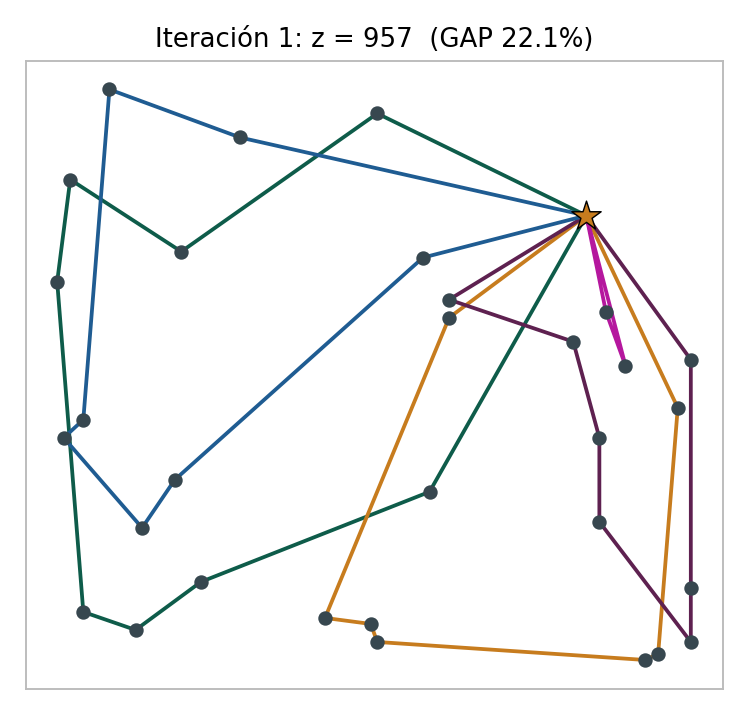
\includegraphics[width=0.8\linewidth]{figuras/evolucion_iter001.png}\\[1pt]
{\scriptsize \azul{\textbf{Iteración 1}}: rutas cruzadas (GAP 22\%).}
\column{0.33\textwidth}\centering
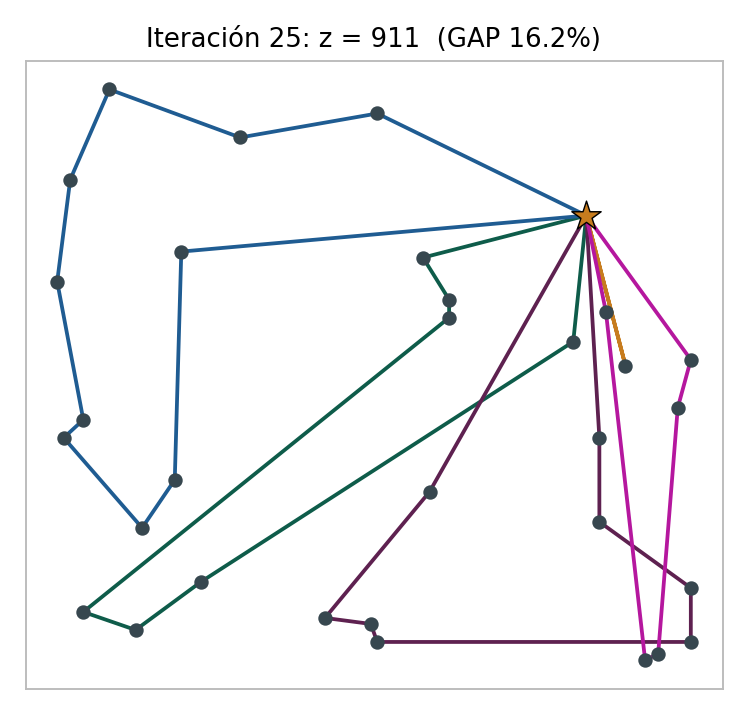
\includegraphics[width=0.8\linewidth]{figuras/evolucion_iter025.png}\\[1pt]
{\scriptsize \azul{\textbf{Iteración 25}}: \naranja{lo social} ordena sectores (GAP 16\%).}
\column{0.33\textwidth}\centering
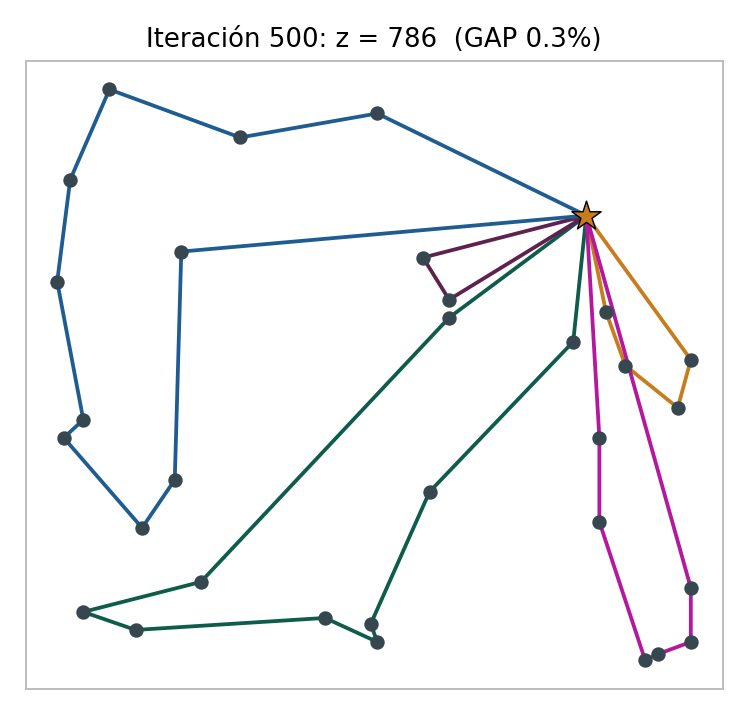
\includegraphics[width=0.8\linewidth]{figuras/evolucion_iter500.png}\\[1pt]
{\scriptsize \azul{\textbf{Iteración 500}}: rutas limpias (GAP 0,26\%).}
\end{columns}
\vspace{2pt}
\begin{ideaclave}
\scriptsize
El mejor global, \textbf{decodificado a rutas}, pasa de un ovillo aleatorio a $0{,}26\%$ del óptimo en $\approx 0{,}1$ segundos.
\end{ideaclave}
\end{frame}

\begin{frame}{Rutas finales: óptimo certificado vs.\ mejor PSO}
\centering
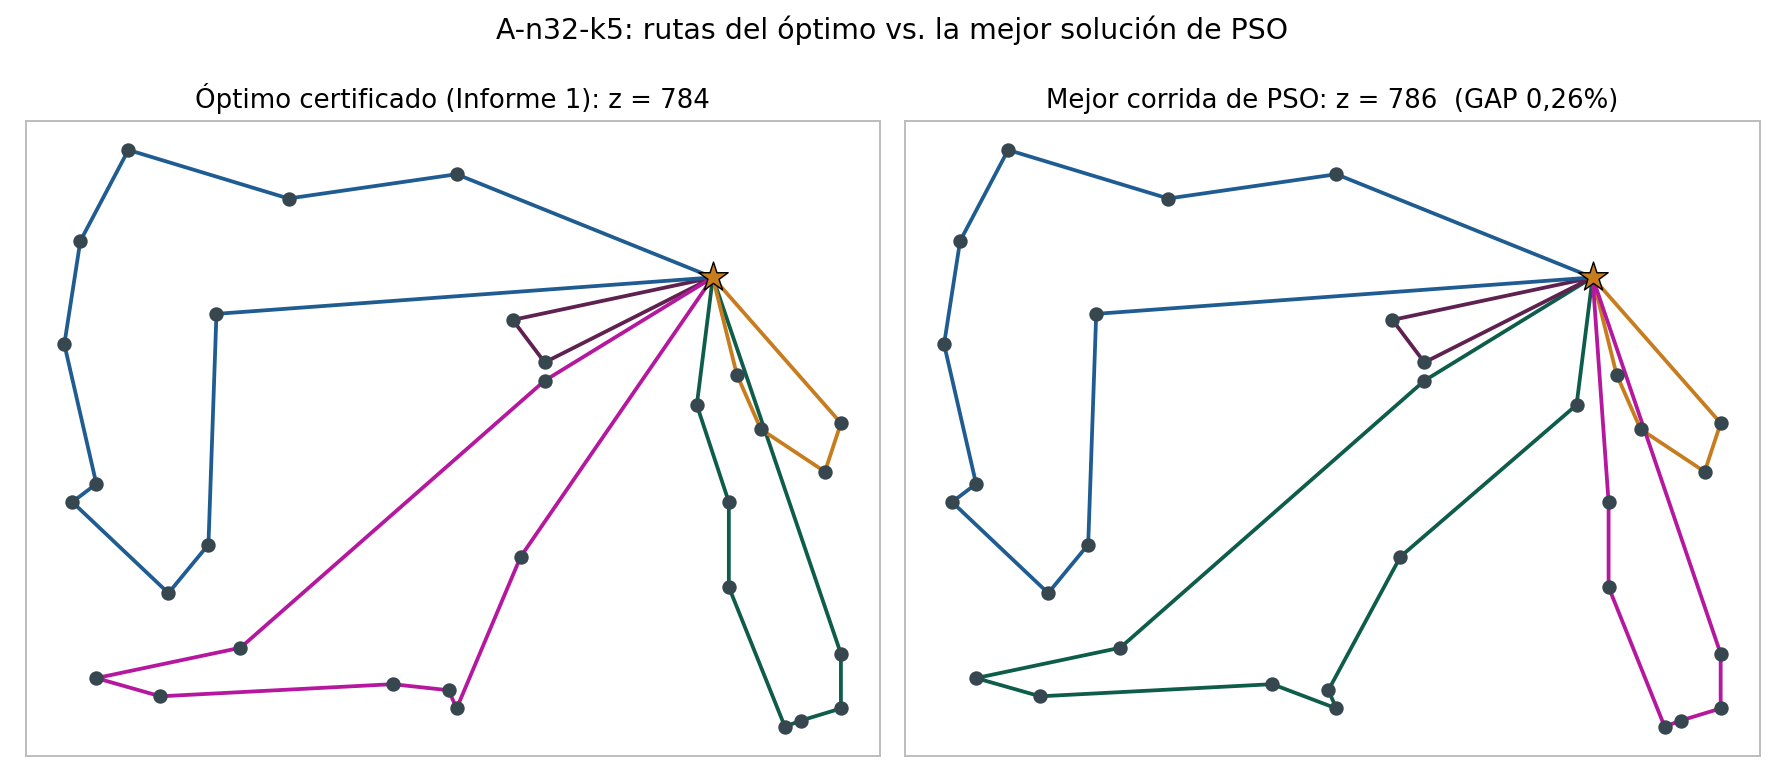
\includegraphics[width=0.72\linewidth]{figuras/rutas_opt_vs_pso.png}
\vspace{2pt}
\begin{ideaclave}
\scriptsize
Rutas \textbf{casi indistinguibles}: misma sectorización, pequeñas diferencias de orden interno ($784$ vs.\ $786$, GAP $0{,}26\%$).
\end{ideaclave}
\end{frame}

\begin{frame}{Calidad de solución: GAP\% por instancia (31 corridas)}
\centering
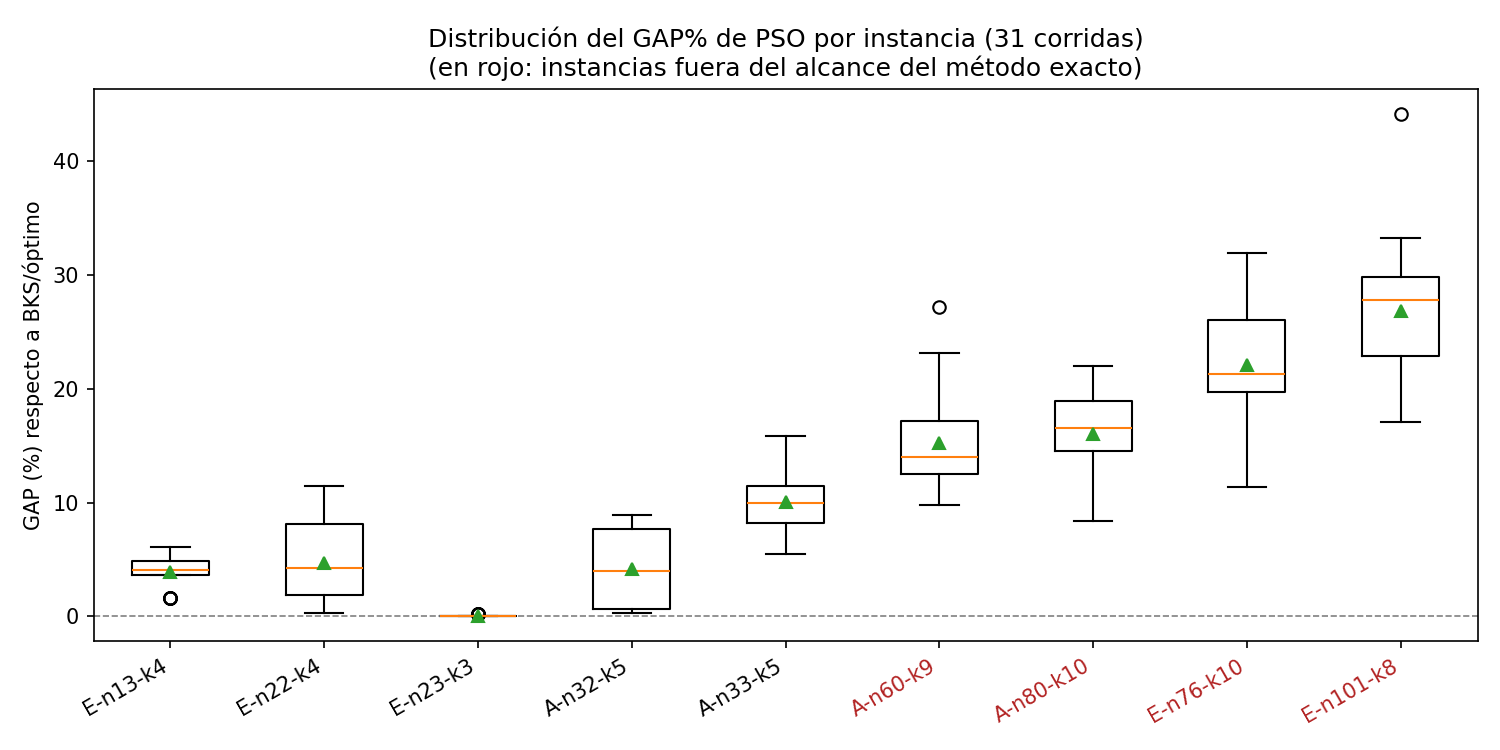
\includegraphics[width=0.76\linewidth]{figuras/boxplot_gap_pso.png}
\vspace{2pt}

{\scriptsize \azul{\textbf{Compartidas}} ($n\le33$): GAP promedio $0{,}03\%$--$10{,}07\%$, toca el óptimo en \texttt{E-n23-k3}. \quad \naranja{\textbf{Escalabilidad}} ($n\ge60$): $15{,}25\%$--$26{,}84\%$, crece al salir del rango de tuning.}
\end{frame}

\begin{frame}{Convergencia: el presupuesto sobra en las chicas, apenas alcanza en las grandes}
\centering
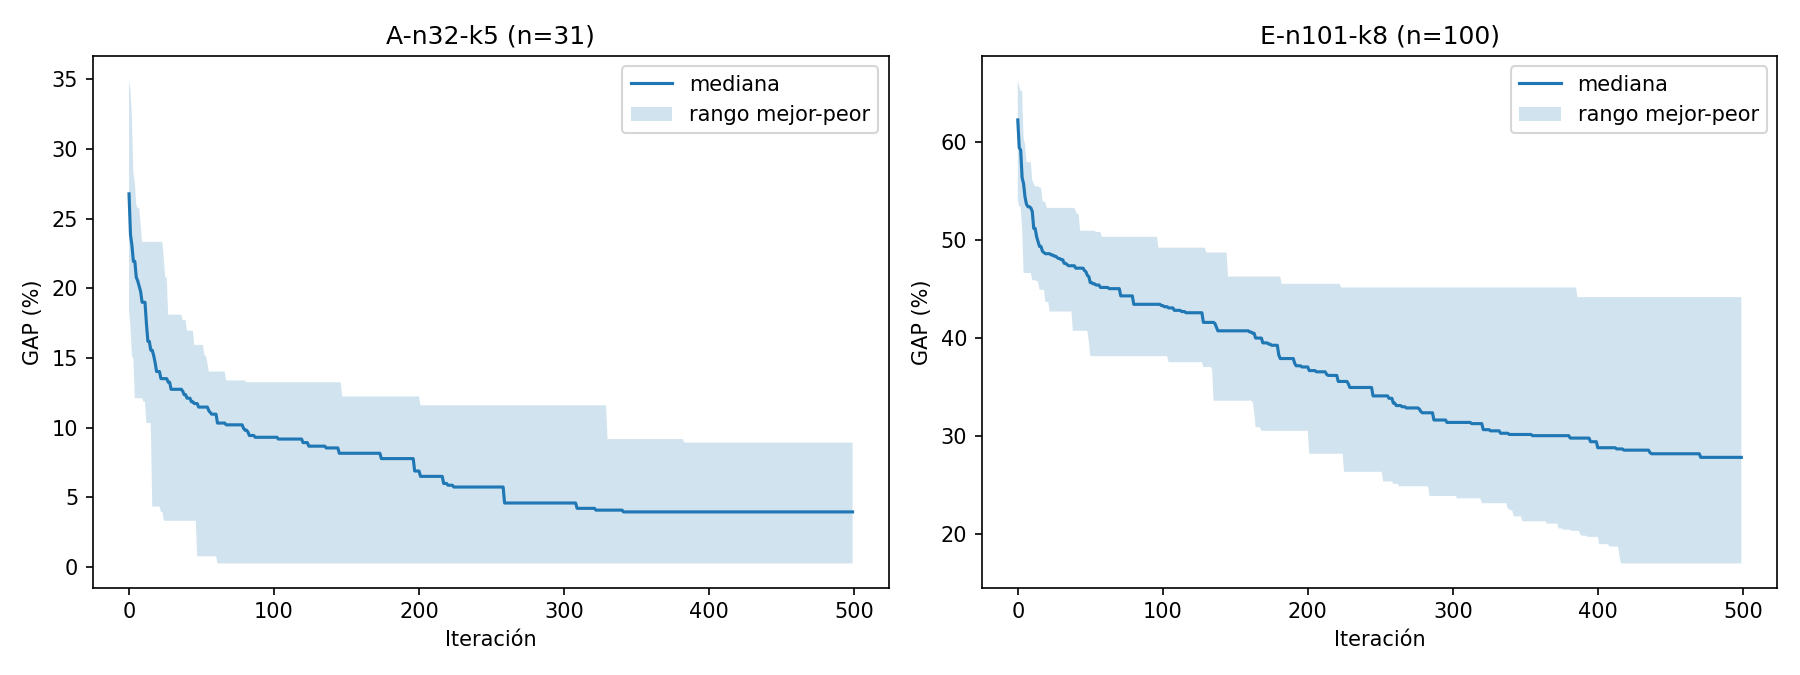
\includegraphics[width=0.78\linewidth]{figuras/convergencia_comparacion.png}
\vspace{2pt}
\begin{ideaclave}
\scriptsize
En \texttt{A-n32-k5} la mediana deja de mejorar en la iteración \textbf{341} de 500; en \texttt{E-n101-k8} sigue mejorando hasta la \textbf{471}.
\end{ideaclave}
\end{frame}

\begin{frame}{Tiempo de resolución: el acantilado del método exacto}
\centering
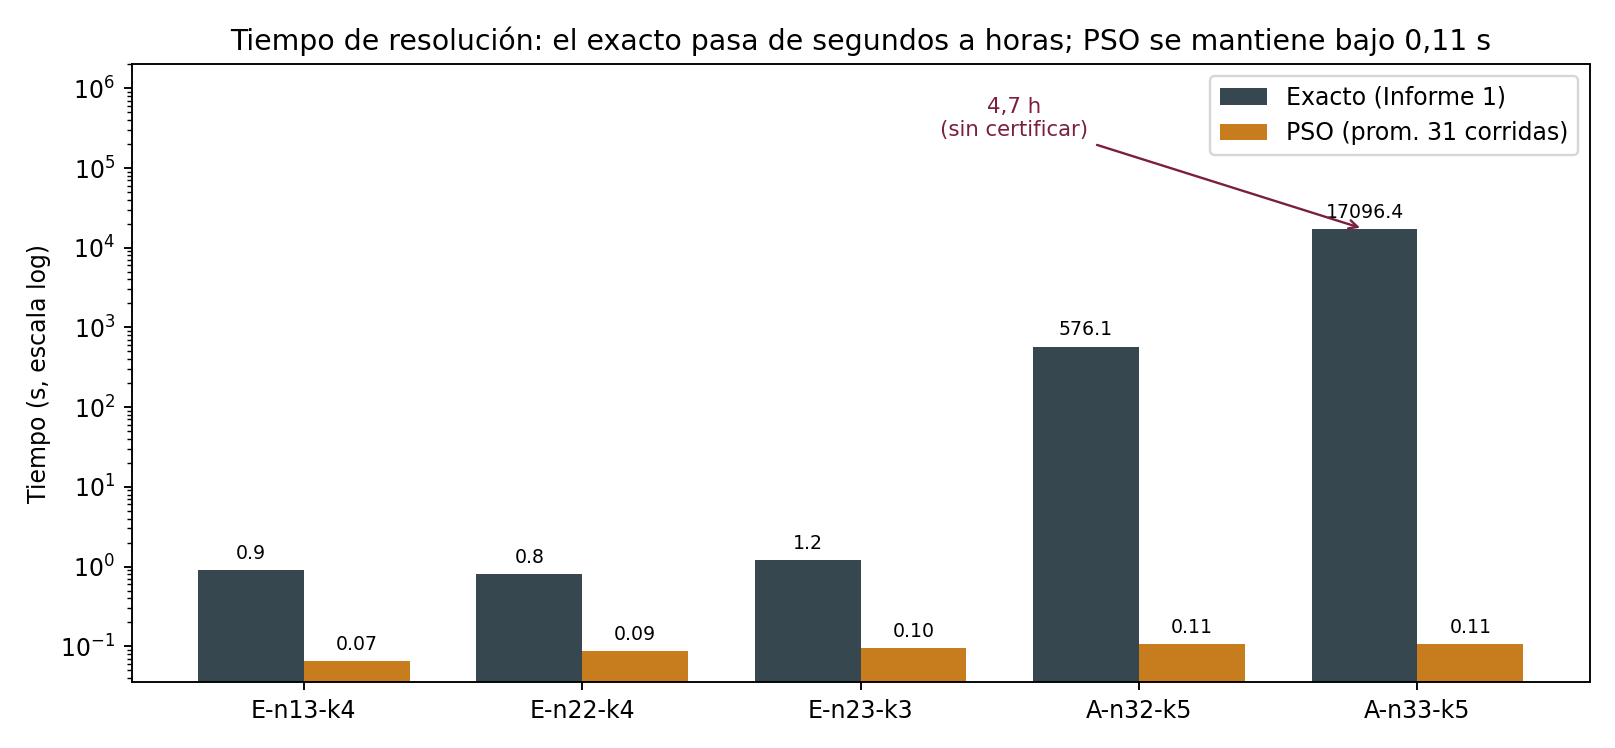
\includegraphics[width=0.74\linewidth]{figuras/acantilado_tiempo.png}
\vspace{2pt}
\begin{ideaclave}
\scriptsize
Mismo equipo para ambos métodos. En \texttt{A-n32-k5} PSO es $\approx 5\,460\times$ más rápido; en \texttt{A-n33-k5}, $\approx 161\,000\times$.
\end{ideaclave}
\end{frame}

\begin{frame}{La comparación completa: PSO converge antes de que el exacto despegue}
\centering
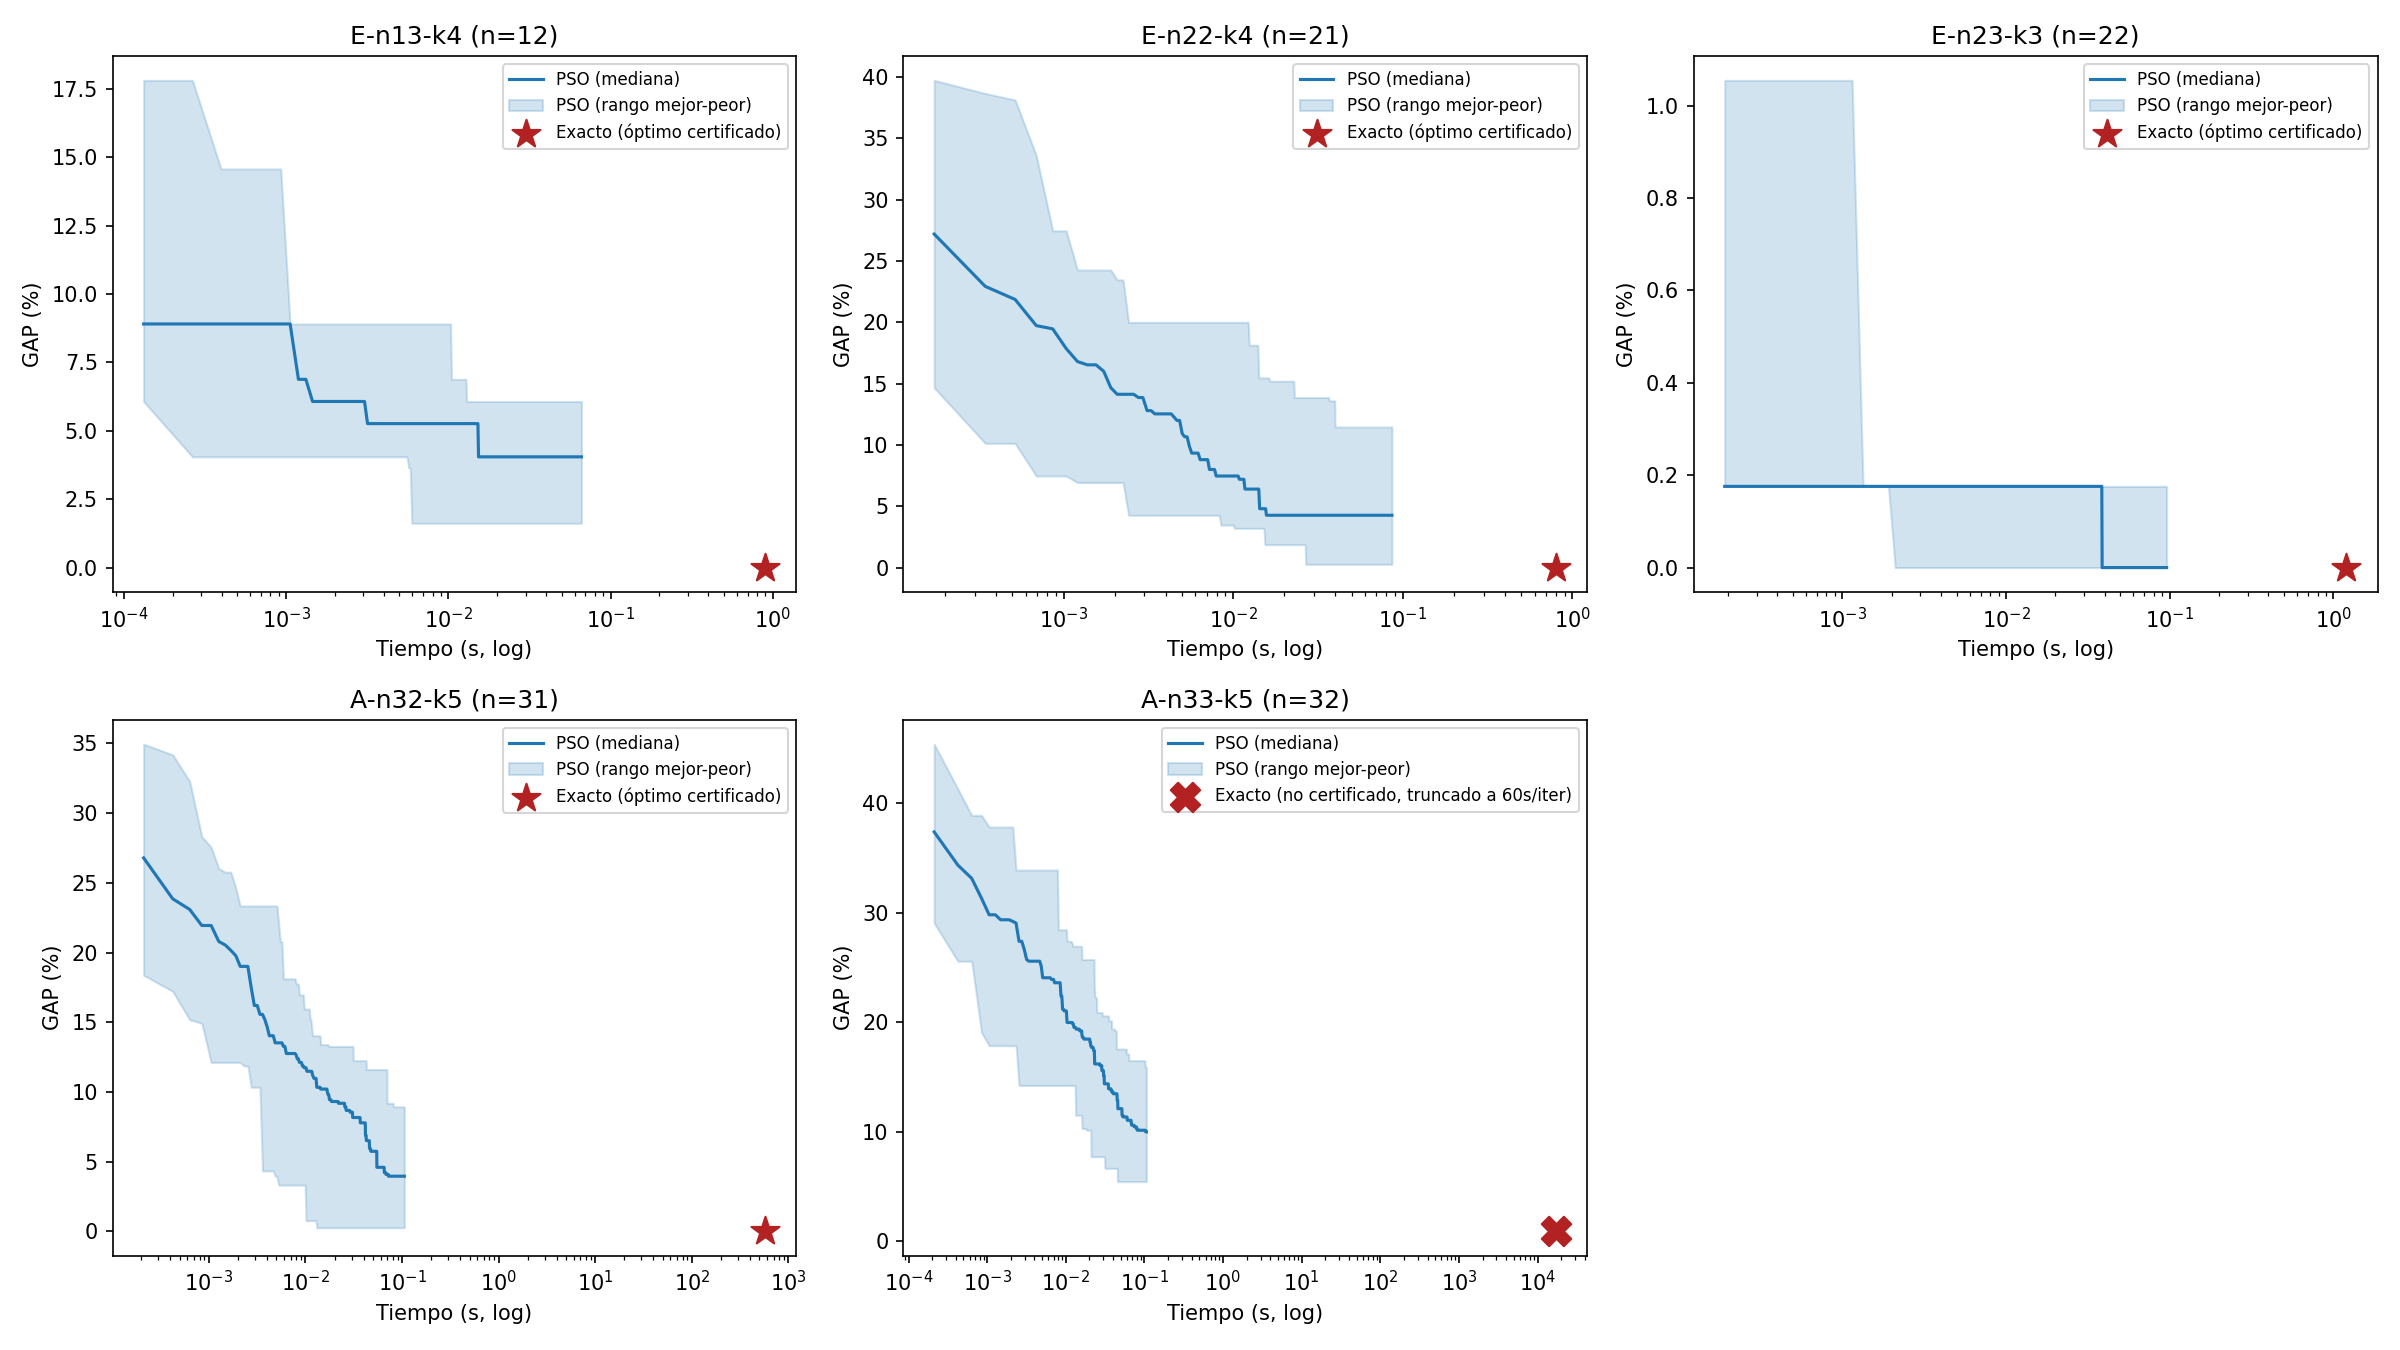
\includegraphics[width=0.66\linewidth]{figuras/convergencia_tiempo_exacto_vs_pso.png}
\vspace{1pt}

{\scriptsize El exacto se reporta como un \textbf{punto} ($\star$ óptimo certificado, $\times$ truncado sin certificar). Eje de tiempo en \textbf{escala log}.}
\end{frame}

% =====================================================================
\section{Conclusiones}
% =====================================================================

\begin{frame}{Conclusiones: los dos métodos, cara a cara}
\vspace{6pt}
\begin{columns}[c]
\column{0.46\textwidth}
\begin{block}{Método exacto}
\footnotesize
\begin{itemize}\setlength\itemsep{6pt}
  \item \azul{Certifica optimalidad}: preferible sin ambigüedad mientras sea tratable.
  \item Pero la tratabilidad se pierde \textbf{de golpe}: $n{=}32\to33$ pasó de minutos a 4,7\,h sin certificado.
\end{itemize}
\end{block}
\column{0.04\textwidth}
\column{0.46\textwidth}
\begin{alertblock}{PSO (SR-1)}
\footnotesize
\begin{itemize}\setlength\itemsep{6pt}
  \item Sin certificado, pero \naranja{tiempo acotado y predecible} ($\le 0{,}31$\,s hasta $n{=}101$).
  \item GAP $\le 5\%$ cerca del rango de tuning; hasta $27\%$ al alejarse de él.
\end{itemize}
\end{alertblock}
\end{columns}
\vspace{14pt}
\begin{ideaclave}
\footnotesize
La conclusión central es la \textbf{complementariedad}, no la sustitución: \azul{el exacto certifica pero no escala; PSO escala pero no certifica.}
\end{ideaclave}
\end{frame}

\begin{frame}{Conclusiones: hallazgos específicos de este trabajo}
\footnotesize
Más allá de la dicotomía general, los datos revelan cuatro observaciones concretas:
\vspace{4pt}
\begin{enumerate}\setlength\itemsep{6pt}
  \item \azul{\textbf{El acantilado es abrupto, no una pendiente.}} Un solo cliente más ($n{=}32\to33$) multiplicó el tiempo del exacto por $\approx 30$ ($576$\,s $\to$ $4{,}7$\,h) y aun así \textbf{no certificó}: la intratabilidad aparece de golpe.
  \item \azul{\textbf{Donde ambos aplican, certificar aporta poco a la \emph{calidad}.}} En 4 de las 5 instancias compartidas PSO quedó a $<5\%$ del óptimo real, en \emph{miles} de veces menos tiempo: el certificado del exacto vale por la garantía, no por una mejora tangible de calidad ahí.
  \item \azul{\textbf{La dificultad de PSO no depende solo de $n$.}} \texttt{E-n76-k10} (GAP $22\%$) resultó más difícil que \texttt{A-n80-k10} (GAP $16\%$) pese a ser más chica: pesa la \naranja{estructura} de la instancia (razón demanda/capacidad, familia), no solo su tamaño.
  \item \azul{\textbf{El presupuesto fijo de evaluaciones es un arma de doble filo.}} Sobra en instancias chicas (\texttt{A-n32-k5} converge en la iteración $341/500$) y falta en las grandes (\texttt{E-n101-k8} aún mejora en la $471/500$).
\end{enumerate}
\end{frame}

\begin{frame}{Conclusiones: recomendación y trabajo futuro}
\begin{ideaclave}
\footnotesize
\textbf{Recomendación práctica:} usar el \azul{método exacto} mientras la instancia caiga antes del acantilado ($n\lesssim 32$ en este banco), donde es rápido y certifica; a partir de ahí, \naranja{PSO} es la única de las dos opciones que devuelve una solución usable en tiempo acotado.
\end{ideaclave}
\vspace{6pt}
\begin{paperbox}
\footnotesize
\textbf{Trabajo futuro} (derivado directamente de los hallazgos anteriores):
\begin{itemize}\setlength\itemsep{4pt}
  \item Variante \textbf{GLNPSO} con vecindario social (\textit{lbest}/\textit{nbest}) para cerrar la brecha de GAP frente a la literatura (hallazgo 2).
  \item \textbf{Escalar} el número de iteraciones con la dimensión $n{+}2m$, en vez de fijarlo por presupuesto (hallazgo 4).
  \item Ampliar el \textbf{tuning} a todo el rango de tamaños y estructuras evaluadas (hallazgos 3 y 4).
\end{itemize}
\end{paperbox}
\end{frame}

% =====================================================================
\section{Referencias}
% =====================================================================

\begin{frame}{Referencias}
\scriptsize
\begin{columns}[T]
\column{0.5\textwidth}
\textbf{Problema y método exacto (Informe 1)}\par\smallskip
Laporte, G., \& Nobert, Y. (1983). A branch and bound algorithm for the capacitated vehicle routing problem. \emph{Operations Research Spektrum, 5}(2), 77--85.\par\smallskip
Lysgaard, J., Letchford, A. N., \& Eglese, R. W. (2004). A new branch-and-cut algorithm for the capacitated vehicle routing problem. \emph{Mathematical Programming, 100}, 423--445.\par\smallskip
Toth, P., \& Vigo, D. (Eds.). (2002). \emph{The Vehicle Routing Problem}. SIAM.\par\smallskip
CVRPLIB (2024). \emph{Capacitated Vehicle Routing Problem Library}. \texttt{vrp.atd-lab.inf.puc-rio.br}.
\column{0.5\textwidth}
\textbf{Metaheurística: PSO (Informe 2)}\par\smallskip
Kennedy, J., \& Eberhart, R. (1995). Particle swarm optimization. \emph{Proc.\ IEEE ICNN}, 1942--1948.\par\smallskip
Shi, Y., \& Eberhart, R. (1998). A modified particle swarm optimizer. \emph{Proc.\ IEEE CEC}, 69--73.\par\smallskip
Clerc, M., \& Kennedy, J. (2002). The particle swarm: explosion, stability, and convergence. \emph{IEEE Trans.\ Evol.\ Comput., 6}(1), 58--73.\par\smallskip
Poli, R., Kennedy, J., \& Blackwell, T. (2007). Particle swarm optimization: An overview. \emph{Swarm Intelligence, 1}(1), 33--57.\par\smallskip
Ai, T. J., \& Kachitvichyanukul, V. (2009). Particle swarm optimization and two solution representations for solving the CVRP. \emph{Computers \& Industrial Engineering, 56}(1), 380--387.
\end{columns}
\vspace{4pt}
{\tiny \gris{\textbf{Herramientas:} Harris et al.\ (2020), \emph{NumPy}, Nature 585, 357--362; Lam et al.\ (2015), \emph{Numba}, Proc.\ LLVM-HPC; Akiba et al.\ (2019), \emph{Optuna}, Proc.\ ACM SIGKDD, 2623--2631.}}
\end{frame}

% ─── CIERRE ──────────────────────────────────────────────────────────
\begin{frame}[plain]
\vfill\begin{center}
{\Huge\bfseries\azul{Gracias}}\\[10pt]
{\large ¿Preguntas?}\\[18pt]
\footnotesize
Cristopher Angulo Ahumada\\[4pt]
\gris{Código y datos: \texttt{github.com/OrejiNet/CVRP-Exact-Method-vs-Particle-Swarm-Optimization}}
\end{center}\vfill
\end{frame}

% =====================================================================
% ─── APÉNDICE ────────────────────────────────────────────────────────
% =====================================================================
\appendix

\begin{frame}[noframenumbering]{Apéndice: resultados completos de PSO (31 corridas por instancia)}
\centering
\footnotesize
\setlength{\tabcolsep}{6pt}
\begin{tabular}{@{}lrrrrrrr@{}}
\toprule
\textbf{Instancia} & $n$ & \textbf{Ref.} & \textbf{Mejor} & \textbf{Prom.} & \textbf{Desv.} & \textbf{Gap prom.\ (\%)} & \textbf{t (s)} \\
\midrule
E-n13-k4  & 13  & 247  & 251  & 256{,}6  & 3{,}0  & 3{,}89  & 0{,}066 \\
E-n22-k4  & 22  & 375  & 376  & 392{,}5  & 12{,}3 & 4{,}66  & 0{,}086 \\
E-n23-k3  & 23  & 569  & 569  & 569{,}2  & 0{,}4  & 0{,}03  & 0{,}096 \\
A-n32-k5  & 32  & 784  & 786  & 816{,}7  & 25{,}4 & 4{,}17  & 0{,}106 \\
A-n33-k5  & 33  & 661  & 697  & 727{,}6  & 16{,}2 & 10{,}07 & 0{,}106 \\
\midrule
A-n60-k9   & 60  & 1354 & 1486 & 1560{,}5 & 56{,}3 & 15{,}25 & 0{,}172 \\
E-n76-k10  & 76  & 830  & 924  & 1013{,}2 & 40{,}3 & 22{,}07 & 0{,}212 \\
A-n80-k10  & 80  & 1763 & 1911 & 2045{,}4 & 71{,}3 & 16{,}02 & 0{,}226 \\
E-n101-k8  & 101 & 815  & 954  & 1033{,}7 & 44{,}2 & 26{,}84 & 0{,}306 \\
\bottomrule
\end{tabular}
\vspace{4pt}

{\scriptsize Presupuesto: 50\,000 evaluaciones por corrida; semillas $0,\ldots,30$. Núcleo de decodificación acelerado con Numba ($\sim$130\,000--200\,000 evaluaciones/s).}
\end{frame}

\begin{frame}[noframenumbering]{Apéndice: espacio de búsqueda de la parametrización}
\centering
\footnotesize
\setlength{\tabcolsep}{8pt}
\begin{tabular}{@{}lll@{}}
\toprule
\textbf{Parámetro} & \textbf{Rango explorado} & \textbf{Óptimo (Optuna)} \\
\midrule
$N$ (partículas) & $\{20, 30, 50, 80, 100\}$ & $100$ \\
$w_0$ & $[0{,}5,\ 0{,}95]$ & $0{,}9116$ \\
$w_f$ & $[0{,}1,\ 0{,}5]$ & $0{,}2782$ \\
$c_1$ & $[0{,}5,\ 2{,}5]$ & $2{,}4045$ \\
$c_2$ & $[0{,}5,\ 2{,}5]$ & $1{,}1843$ \\
$v_{\max}$ (fracción) & $[0{,}1,\ 1{,}0]$ & $0{,}3762$ \\
\bottomrule
\end{tabular}
\vspace{4pt}

{\scriptsize Muestreador TPE; 60 \textit{trials} ($\approx 10\times$ el número de hiperparámetros); $T=\lfloor 50\,000/N \rfloor$ para igualar esfuerzo entre configuraciones. Instancias de tuning: \texttt{A-n34-k5} (GAP $3{,}34\%$), \texttt{A-n62-k8} ($7{,}92\%$), \texttt{E-n76-k7} ($14{,}37\%$).}
\end{frame}

\end{document}
